        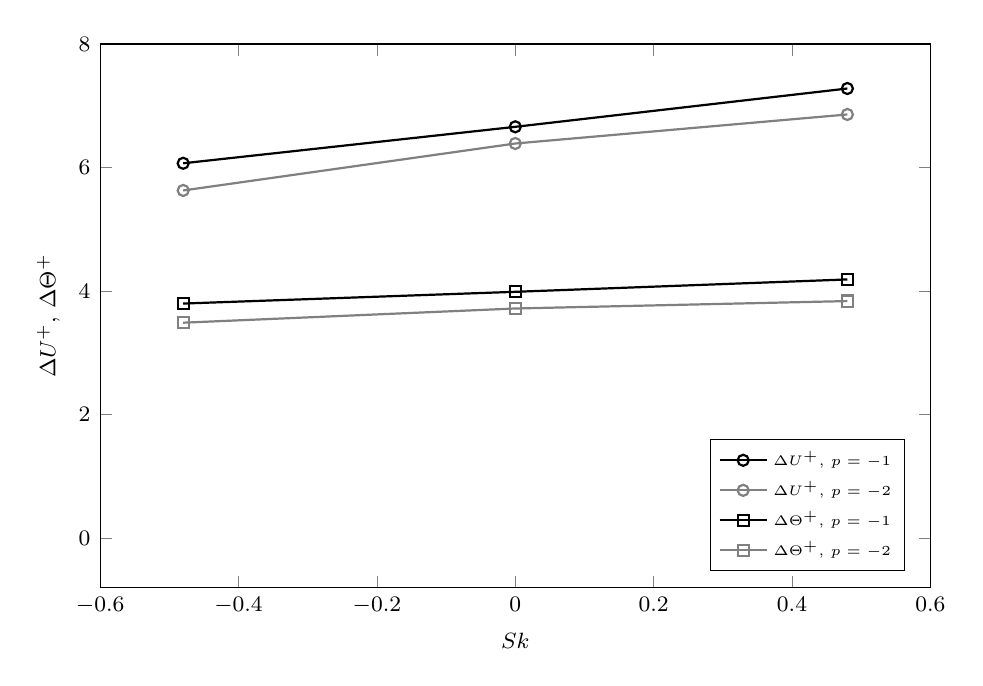
\begin{tikzpicture}
        \centering
        \begin{axis}[
            ylabel={$\Delta U^+$, $\Delta \Theta^+$},
            xlabel={$Sk$},
            ymin=-0.8, ymax=8,
			xmax=0.6,
			xmin=-0.60,
					ylabel near ticks,
            width=1\linewidth,
            height=0.7\linewidth,
            label style={font=\footnotesize},
            legend style={font=\tiny,anchor=south east},
                        legend pos=south east,
            tick label style={font=\footnotesize}
            ]
			\addplot [
            black,thick,mark=o,
            ]
            coordinates{
            (0.48, 7.28)
            (0, 6.66)
            (-0.48,6.07)
            };
			\addlegendentry{$\Delta U^+$, $p=-1$}
						\addplot [
            gray,thick,mark=o,
            ]
            coordinates{
            (0.48, 6.86)
            (0, 6.39)
            (-0.48,5.63)
            };
			\addlegendentry{$\Delta U^+$, $p=-2$}
					\addplot [
            black,thick,mark=square,
            ]
            coordinates{
            (0.48, 4.19)
            (0, 3.99)
            (-0.48,3.80)
            };
			\addlegendentry{$\Delta \Theta^+$, $p=-1$}
						\addplot [
            gray,thick,mark=square,
            ]
            coordinates{
            (0.48, 3.84)
            (0, 3.72)
            (-0.48,3.49)
            };
			\addlegendentry{$\Delta \Theta^+$, $p=-2$}
        \end{axis}
        \end{tikzpicture}